\documentclass[notes]{subfiles}
\begin{document}
	\chapter{Derivatives}
	\setcounter{section}{1}
	\addcontentsline{toc}{section}{3.1 - Defining the Derivative}
	\fancyhead[RO,LE]{\bfseries \large \nameref{cs31}} 
	\fancyhead[LO,RE]{\bfseries \currentname}
	\fancyfoot[C]{{}}
	\fancyfoot[LO,RE]{\large \thepage}	%Footer on Right \thepage is pagenumber
	\fancyfoot[RO,LE]{\large Chapter 3.1}

\section*{Defining the Derivative}\label{cs31}
	\subsection*{Before Class}
	\subsubsection*{Tangent Lines \& Secant Lines}
		Recall that the slope of the line between two points on the curve \(f(x)\) is given in a few ways:
			\vspace{1.5in}

		\begin{defn}[Tangent/Secant Lines]
			The \textbf{tangent line} to a curve \(f(x)\) is a line which intersects the curve at \blank{1.5}\\[15pt]  \blank{2.5}.  A \textbf{secant line} intersects a curve \blank{1.7}\\[15pt] \blank{2.5}.
				
		\end{defn}
		Here is a brief illustration of a tangent line and a secant line.
			\newpage
			
		\begin{ex}
			The points \((2,4)\) and \((4,16)\) lie on the graph of \(f(x)\).  
			\begin{enumerate}[(a)]
				\item Find the slope of the secant line between these two points.
					\vs{1}
				\item Find the formula for the secant line between these points.
					\vs{1}
					
				\item Assume \(f(x) = x^2\).  Give a quick sketch of \(f(x)\), along with the points given (you don't have to be super precise).  How ``close'' are we to having a tangent line?  Is there a way to get ``closer'' to having a tangent line?
					\vs{2}
			\end{enumerate}
		\end{ex}
			\newpage
						
		\begin{ex}
			The function \(f(x) = x^2\) is graphed below.\\
			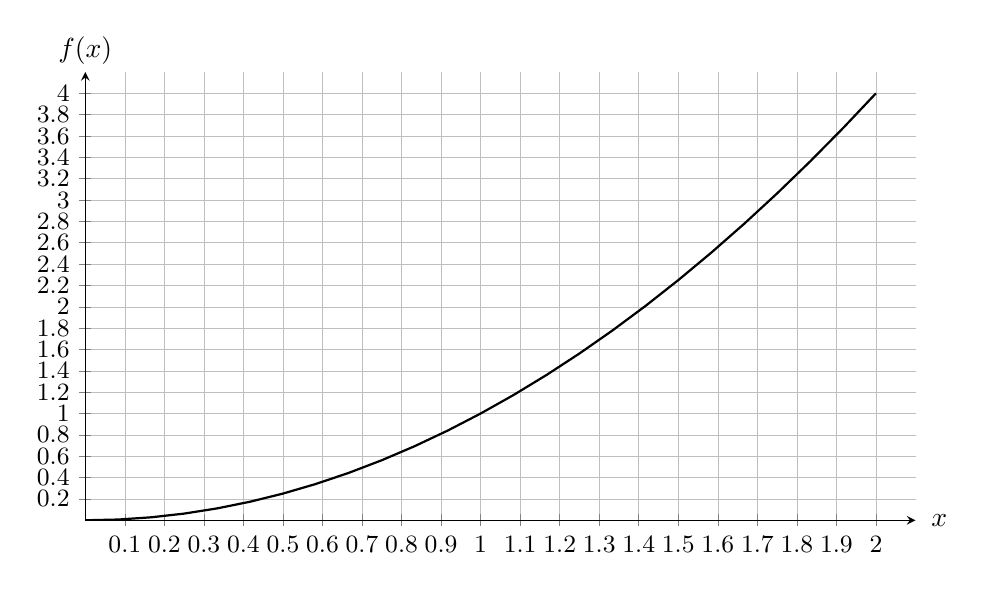
\begin{tikzpicture}
				\begin{axis}[
					grid = both,
					grid style={line width=.1pt, draw=gray!10},
					major grid style={line width=.2pt,draw=gray!50},
					width = \textwidth,
					height = .6\textwidth,
					every tick label/.append style={font=\small},
					axis x line = middle,
					axis y line = left,
		    			every axis y label/.style={at={(ticklabel cs:1.15)}},
						y label style={at={(axis description cs:0,1.1)},anchor=north},
					ytick = {0.2, 0.4,...,4},
		    			ylabel = {$f(x)$},
		    			ymin = 0, ymax = 4.2,
	    				every axis x label/.style= {at ={(ticklabel cs:1)}},
	    				xtick = {0.1, 0.2,...,2},
		    				x label style={at={(axis description cs:1.05,0)},anchor=east},
	    				xlabel = {$x$},
	    				xmin = 0, xmax = 2.1			
				]
					\addplot[thick, domain = 0:2] {x^2};
				\end{axis}
			\end{tikzpicture}\\[10pt]
			Approximate the slope of the tangent line to \(f\) at \(x = 1\) by finding the slope of the secant line through \((1,1)\) and the following points.  Sketch a few secant lines on the graph above as well.
			\begin{center}
			\begin{multicols*}{2}
				\begin{enumerate}[(a)]
					\setlength\itemsep{1.25in}
					\item \((0.7, 0.49)\)
						
					\item \((0.8, 0.64)\)
						 							
					\item \((0.9, 0.81)\)
						\columnbreak
											
					\item \((1.3, 1.69)\)
						 							
					\item\((1.2, 1.44)\)
						 							
					\item \((1.1, 1.21)\)

				\end{enumerate}
					\raggedcolumns
			\end{multicols*}
			\end{center}
		\end{ex}
			\newpage
			
	\subsubsection*{Transitioning to the Derivative}
	
		\begin{defn}[Slope of the Tangent Line 1]
			The \textbf{tangent line} to a curve \(y = f(x)\) at the point \(P(a,f(a))\) is the line through the point \(P\) with slope
			
				\\ \vspace{.75in}
			
			provided that this limit exists.
		\end{defn}
		Here are some pictures to help give some intution to the definition:

			\vspace{2in}
			
		\begin{ex}
			Find the slope of the secant line through the points \((a,f(a))\) and \((a+h,f(a+h))\)
		\end{ex}
			\vs{1}
			\newpage
			
		\begin{defn}[Slope of the Tangent Line 2]
			The \textbf{tangent line} to a curve \(y = f(x)\) at the point \(P(a,f(a))\) is the line through the point \(P\) with slope
			
				\\ \vspace{.75in}
			
			provided that this limit exists, where \(h\) is considered to be a \\ \\[5pt]
			
				\blank{3.5}.
			
		\end{defn}
		Here are some more pictures for the new defintion:
			\vs{1}
			
	\subsubsection*{Tangents \& Velocities}
		
		Suppose we want to find the average velocity of an object.  We can use the same approach as we did above to find this.  The average velocity of an object is given by
			\[v_{avg} = \dfrac{\text{change in position}}{\text{change in time}}\]
			
		\begin{ex}
			Rewrite the expression for average velocity in a way similar to how we wrote the expressions for secant lines
		\end{ex}
			\vs{1}
			\newpage
		
		\begin{rmk}[Instantaneous Velocity]
			The \emph{instantaneous velocity} of an object, given its position function \(f(x)\), is
			
				\\ \( \)\vspace{.55in} 
		\end{rmk}	
		
		\begin{ex}
			Suppose that a ball is dropped from the upper observation deck of a building which is 980 m above the ground.
			\begin{enumerate}[(a)]
				\item What is the velocity of the ball after 10 seconds?  Use that the equation of motion is \(s(t) = 4.9t^2\).
					\vs{1}
				\item How fast is the ball traveling when it hits the ground?
					\vs{1}
			\end{enumerate}
		\end{ex}
			\newpage
			
	\subsection*{Pre Class Practice}
		\begin{ex}
			We have two definitions of the slope of a tangent line at an input, \(x = a\).  Rewrite them here.
		\end{ex}
			\vs{1}
			
		\begin{ex}
			Let \(f(x) = x^2 + 1\) and \(a = 3\). Using either definition that you wrote above, show that the slope of the tangent line to \(f(x)\) at \(x=3\) is 6.
		\end{ex}
			\vs{1.5}
		
		\begin{ex}
			A function \(f(x)\) is graphed, along with several tangent lines.  Identify the slope of the tangent line at the points \(x = -3\) and \(x = 2\)
			\begin{flushleft}
				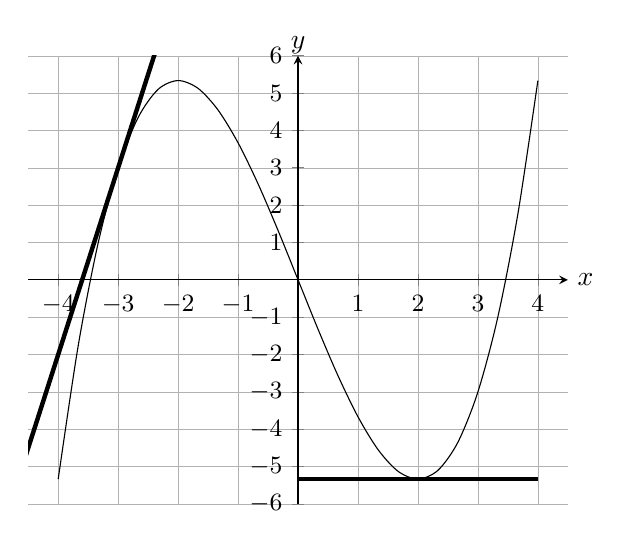
\begin{tikzpicture}
					\begin{axis}[
							grid style = {line width = .1pt, draw = gray!60},
							grid = both,
							every tick label/.append style={font=\small},
							axis x line = middle,
							axis y line = middle,
				    			every axis y label/.style={at={(ticklabel cs:1.15)}, yshift = -3pt},
								y label style={at={(axis description cs: 0.5, 1)},above},
							ytick = {-10,-9,-8,-7,-6,-5,-4,-3,-2,-1,1,2,3,4,5,6,7,8,9,10},
				    			ylabel = {$y$},
				    			ymin = -6, ymax = 6,
			    				every axis x label/.style= {at ={(ticklabel cs:1)}},
			    				xtick = {-4,-3,-2,-1,1,2,3,4},
				    				x label style={at={(axis description cs: 1, 0.5)},right},
			    				xlabel = {$x$},
			    				xmin = -4.5, xmax = 4.5			
						]
						\addplot[smooth,domain = -4:4] {(1/3)*x^3 - 4*x};
						\addplot[smooth, ultra thick, domain = 0:4] {-16/3};
						\addplot[smooth, ultra thick, domain = -6:0] {5*x + 18};
					\end{axis}
				\end{tikzpicture}
			\end{flushleft}
		\end{ex}
			\newpage
			
	\subsection*{In Class}	
	\subsubsection*{Derivatives}
		\begin{defn}[The Derivative (at \(x = a\))]
			The \textbf{derivative of a function} \(f\) at input \(x = a\) is given by

				\\ \vspace{.5in}
			
			or
				\\ \vspace{.5in}
			
			if this limit exists.
		\end{defn}
			
		We have two ways of interpreting what the derivative actually means:\\
			\begin{itemize}
			\setlength\itemsep{15pt}
				\item The derivative \(f'(a)\) is the \blank{4.5}\\[15pt] \blank{4}.
				\item The derivative \(f'(a)\) is \blank{5} \\[15pt] \blank{3}.
			\end{itemize}
		
		\begin{ex}
			Let \(f(x) = x^2\).  Show that \(f'(1) = 2\) using \emph{both} formulas for the derivative at a point.
		\end{ex}
			\vs{1}
			\newpage
			
		\begin{ex}
			\begin{enumerate}[(a)]
				\item Use both definitions of the derivative at a point to show that for \(f(x) = x^3\), \(f'(1) = 3\).
					\vs{1.5}
					
				\item Find the equation of the tangent line to \(f(x)\) at the point \(x = 1\).
					\vs{1}
					
			\end{enumerate}
		\end{ex}
			
		\begin{ex}
			Find the derivative of the function \(f(x) = x^2-6x+1\) at the input \(x = a\).
		\end{ex}
			\vs{2}
			\newpage
			
		\begin{ex}
			Find the equation of the tangent line to the parabola \(y = x^2 + 4x\) at the point \((-1,-3)\).
		\end{ex}
			\vs{2}
			
		\begin{ex}
			Find an equation of the tangent line to the graph of \(y = h(x)\) at \(x = 5\) if \(h(5) = -3\) and \(h'(5) = 4\).
		\end{ex}
			\vs{1}
			
		\begin{ex}
			If \(\ds f'(a) = \lim_{h\to 0} \dfrac{\sqrt{16 + h} - 4}{h}\) represents the derivative of the function \(f(x)\) at \(x = a\), what is \(f(x)\) and what is \(a\)?
		\end{ex}
			\vs{1}
			\newpage
			
		\begin{ex}
			The function \(C\) gives the number of bushels of corn produced on a tract of farmland that is treated with \(f\) pounds of nitrogen per acre.
			\begin{enumerate}[(a)]
				\item Is it possible for \(C(90)\) to be negative?  Why or why not?
					\vs{1}
					
				\item What are the units on \(C'(90)\)?
					\vs{.5}

				\item Is it possible for \(C'(90)\) to be negative?  Why or why not?
					\vs{1}
			\end{enumerate}
		\end{ex}
			
		\begin{ex}
			The function \(p\) gives the number of miles from an airport that a plane has flown after \(t\) hours.
			\begin{enumerate}[(a)]
				\item What are the units of \(p'(1.5)\)?
					\vs{1}
					\newpage
					
				\item What is the common word used for \(p'(1.5)\)?
					\vs{1}
			\end{enumerate}
		\end{ex}

		\begin{ex}
			The cost of producing \(x\) ounces of gold from a new gold mine is \(C=f(x)\) dollars.
			\begin{enumerate}[(a)]
				\item What is the meaning of the derivative \(f'(x)\)?  What are its units?
					\vs{1}
				\item Interpret the statement \(f'(800) = 17\).
					\vs{1}
			\end{enumerate}
		\end{ex}
			\newpage
			
	\subsection*{After Class Practice}
		\begin{ex}
			The tangent line to \(y = f(x)\) at \((3,4)\) passes through the point \((0,2)\).  Find \(f(3)\) and \(f'(3)\).
		\end{ex}
			\vs{1}
			
		\begin{ex}
			Sketch the graph of a function \(g\) for which \(g(0) = g(2) = g(4) = 0\), \(g'(1) = g'(3) = 0\), \(g'(0) = g'(4) = 1\), \(g'(2) = -1\), \(\ds \lim_{x\to 5^-} g(x) = \infty\), and \(\ds \lim_{x\to -1^+} g(x) = -\infty\).
		\end{ex}
			\vs{2}
			
		\begin{ex}
			\(\ds \lim_{\theta\to \pi/6} \dfrac{\sin\theta - \frac{1}{2}}{\theta - \pi/6}\) represents the derivative of a function \(f(\theta)\) at some value of \(\theta = a \).  What is \(f(\theta)\) and what is \(a\)?
		\end{ex}	
			\vs{1}
\clearpage
\end{document}